% Flow configuration and data. New physics-first section in the idiom of
% Fukami's "Flow physics" subsection and the PRF "Simulation setup". It (i)
% describes the encounter as a staged cycle (base -> LEV -> arch/TEV -> recovery),
% following Smith et al. 2024 and Odaka et al. 2026; (ii) frames the baseline as
% a limit cycle, following Fukami, Nakao & Taira 2024; (iii) reframes |G|=4 as a
% physical 2D->3D regime change, following the PRF source paper; (iv) defines the
% six observables physically. The implementation-diary split metadata, the sha,
% and the hardware lines from the original Methods are removed.

\subsection{Vortex gust-airfoil interaction}
\label{sec:flow_physics}

\rb{K}{S2-01}{Configuration, solver provenance and the gust parametrisation. The DNS-not-LES and Fukami-as-reference-not-source distinctions live here.}We study a NACA~0012 airfoil at angle of attack $\alpha = 14^\circ$ and chord
Reynolds number $\vRe = 5000$, perturbed by a discrete vortex gust modelled as a
spanwise-oriented Taylor vortex released upstream of the leading edge. The data
analysed here are our own direct numerical simulations of this configuration,
computed with the GPU-enabled spectral-element solver SOD2D
\citep{gasparino2024sod2d} with no subgrid-scale model, so that all scales of the
separated wake are resolved at this Reynolds number. The solver uses an
incompressible, constant-density pressure-projection formulation
($M = 0$; table~\ref{tab:dns_pending}). The configuration and its physical characterisation follow
Fukami, Smith \& Taira \citeyearpar{fukami2025prf}, which is the reference for the
physics, not the source of the data.
The vortex has the azimuthal velocity profile
\begin{equation}
  u_\theta(r) = u_{\theta,\max}\,\frac{r}{R}\,
  \exp\!\left[\tfrac12\!\left(1 - \frac{r^2}{R^2}\right)\right],
  \label{eq:taylor}
\end{equation}
which peaks at the core radius $r = R$ \citep{taylor1918}, and is parametrised by
three scalars: the signed gust ratio $G \equiv u_{\theta,\max}/u_\infty$, the
core diameter $D \equiv 2R/c$, and the offset $Y$ of the vortex centre,
measured normal to the free stream (figure~\ref{fig:geometry}). The release
point is fixed at $2c$ upstream of the leading edge and offset by $Y$, both
measured in axes aligned with the free stream, following
\citet{fukami2025prf} and the chord is pitched by the angle of attack $\alpha$
relative to these axes. The profile and the $(G, D, Y)$
sampling follow the configuration of \citet{fukami2025prf}. The training envelope spans $|G| \in \{0.25, 0.5, 1.0, 1.5, 2.0,
3.0\}$ with $G = 0$ as the undisturbed reference, $D \in \{0.5, 1.0, 1.5\}$
chords, and $Y \in [-0.4, +0.4]$; the value $|G| = 4$ is held out as an
extrapolation boundary, for reasons that are physical and that we return to
below. Convective time $t$ is measured in chords from the vortex release,
$t = 0$, while $t_{\mathrm{imp}}$ denotes the instant at which the vortex centre
reaches the leading edge, near $t/c = 2$ for this configuration; all phase
windows below are referred to $t_{\mathrm{imp}}$.\re

\begin{figure}
  \centering
  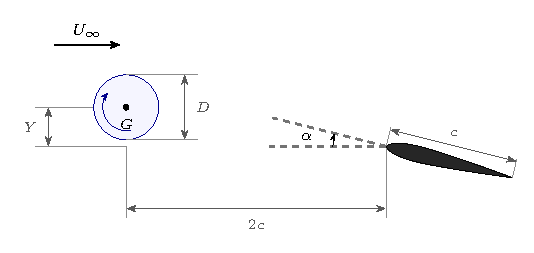
\includegraphics[width=\linewidth]{sections/figures/tikz/fig_case_geometry.pdf}
  \caption{\rb{K}{S2-C1}{Defines the free-stream-aligned axes in which $(G,D,Y)$ are read. Without it the sign conventions of the envelope result are ambiguous.}Case geometry (schematic, not to scale), drawn directly in the
  free-stream-aligned axes in which $(G, D, Y)$ are defined, following
  \citet{fukami2025prf}. The vortex core is released a fixed $2c$ upstream of
  the leading edge (LE), offset by $Y$ normal to the free stream $U_\infty$,
  and convects downstream parallel to it, not along the chord. The chord is
  pitched by the angle of attack $\alpha = 14^\circ$ relative to these axes,
  trailing edge (TE) below leading edge. The core has diameter $D = 2R/c$
  (core radius $R$) and peak azimuthal velocity $u_{\theta,\max}$ setting the
  signed gust ratio $G \equiv u_{\theta,\max}/u_\infty$; the arrow shows the
  clockwise sense of rotation for $G > 0$. Only $(G, D, Y)$ vary across cases.\re}
  \label{fig:geometry}
\end{figure}

\rb{K}{S2-02}{The staged reading of the encounter that the five observables summarise. Physics framing the Results repeatedly refer back to.}Without a gust, the $\alpha = 14^\circ$ wake at this Reynolds number is separated and sheds periodically; in dynamical terms the undisturbed
flow is a limit cycle. A gust encounter is then a transient excursion from this
limit cycle and back, and it is helpful to read it in stages
(figure~\ref{fig:staging}) \citep{smith2024,fukami2025prf,odaka2026}. The vortex
first induces a strong
wall-normal vorticity flux at the leading edge, the airfoil experiences a sharp
lift excursion as a leading-edge vortex (LEV) forms, the LEV rolls up and sheds
together with a trailing-edge structure as the load reaches its extremum, and
the wake then relaxes back toward the baseline shedding. The sign of $G$ sets
whether the first lift excursion is positive or negative, $Y$ sets the side and
strength of the impingement, $D$ sets how much of the encounter is dominated by
the vortex core, and the impact timing sets the phase of the baseline cycle at
which the disturbance arrives. The five observables defined in
\S\ref{sec:flow_observables} are quantitative summaries of exactly this
sequence.\re

\begin{figure}
  \centering
  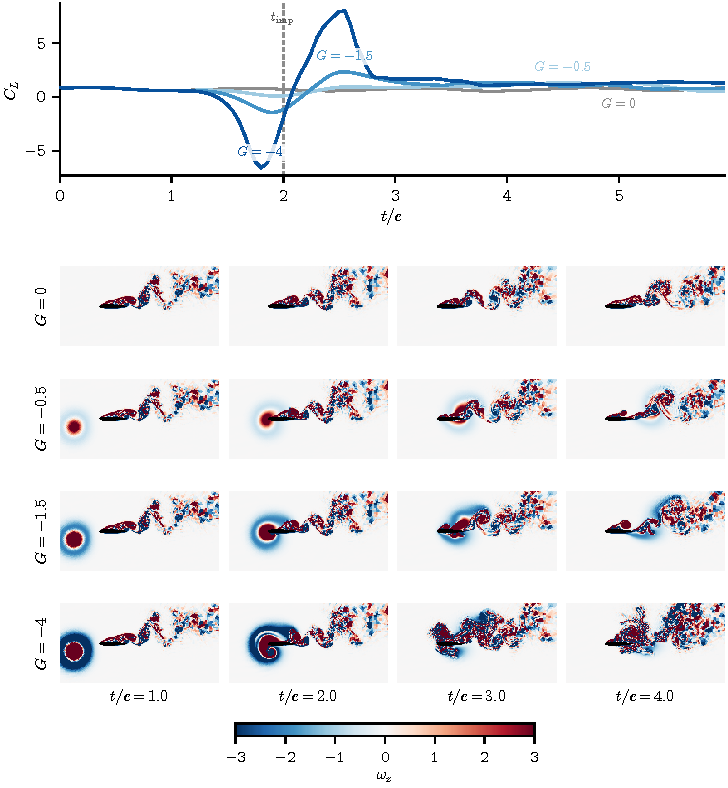
\includegraphics[width=\linewidth]{sections/figures/results/fig_staging_v2p1.pdf}
  \caption{\rb{K}{S2-C2}{The gust-strength sweep that shows the wake reorganisation the paper is about. Also states why the wake, not only $C_L$, is the endpoint.}The vortex gust as a wake-reorganisation event: a gust-strength sweep
  at fixed core diameter $D = 0.5$ and offset $Y = -0.1$ (first encounter of each
  case). Top: lift coefficient $C_L$ against convective time, with $t/c = 0$ the
  release and $t_{\mathrm{imp}}$ (dashed) the leading-edge crossing near
  $t/c = 2$; the load excursion deepens and widens with $|G|$, the baseline
  ($G = 0$) in grey. Bottom: mid-plane spanwise vorticity $\omegaz$ per case (rows
  $G = 0$, $-0.5$, $-1.5$, $-4$) at four times (columns $t/c = 1$, $2$, $3$, $4$),
  raw units, colourbar clipped at $\pm 3$ (intense cores saturate), airfoil
  filled. The strong gust reorganises the wake through impact while the weak cases
  barely perturb the shedding; $G = -4$ is the $|G| = 4$ extrapolation case, shown
  only for illustration. The release parameters alone do not fix where the wake
  sits afterwards, which is why the wake, not only $C_L$, is the endpoint a reduced
  state must carry.\re}
  \label{fig:staging}
\end{figure}

\rb{K}{S2-03}{The physical reason $\lvert G\rvert = 4$ is a regime change and not one parameter step. This paragraph is what licenses the boundary reading in \S4.6, \S5.4 and \S6.}A consequence of the source characterisation \citep{fukami2025prf} is central to
how we read the extrapolation case. For $|G| \le 3$ the encounter is primarily
two-dimensional, so a mid-plane slice of the spanwise vorticity carries the
relevant large-scale dynamics; for $|G| \ge 4$ the interaction becomes
genuinely three-dimensional, with fine-scale instabilities developing during
impact. We confirm this from the full three-dimensional vorticity fields: the
fraction of the spanwise-vorticity ($\omegaz$) enstrophy (the integral of
squared vorticity over a region, formalised for the wake window in
\S\ref{sec:flow_observables}, eq.~\ref{eq:enstrophy}) not captured by its
spanwise mean, the content a mid-plane slice discards, is roughly constant across
the training range ($|G| \le 3$, post-impact wake median $\approx 0.20$) and rises
about threefold at $|G| = 4$ ($\approx 0.56$, computed on the four boundary cases
for which the full three-dimensional fields were retained). Because the encoder
in this work consumes a single mid-plane vorticity
field (\S\ref{sec:flow_observables}), the held-out $|G| = 4$ case is not merely
one parameter step beyond the training range; it is a regime in which the
mid-plane representation omits a substantially larger fraction of the
three-dimensional vorticity content, so that more of the dynamics is not
captured by what the encoder sees. We therefore treat $|G| = 4$ as a physically
more demanding extrapolation set in which a mid-plane state is incomplete, rather
than as a claim of parametric generalisation.\re

\subsection{Data, fields, and observables}
\label{sec:flow_observables}

\rb{K}{S2-04}{Partition, encounter counts and the non-independence caveat behind the case-clustered statistics. Reproducibility rests on it.}Each simulation case is one long run partitioned into encounters of $120$ cached
frames at $\Delta t = 0.05\,t/c$, one encounter per gust release. The
simulations use a spectral-element discretisation of polynomial order $p = 4$,
and the fields are cached on a structured grid of $192 \times 96 \times 32$
points spanning $x/c \in [-1.5, 4.5]$ and $y/c \in [-1.5, 1.5]$ with a spanwise
extent of approximately one chord; this analysis subdomain matches the
data-driven subdomain of the source characterisation \citep{fukami2025prf}. The
lift and drag coefficients are $C_L = F_L/(\tfrac12 \rho u_\infty^2 c)$ and
$C_D = F_D/(\tfrac12 \rho u_\infty^2 c)$, obtained by integrating the pressure
and viscous stresses over the airfoil surface.
The remaining DNS solver-resolution details required for full reproducibility
are listed in table~\ref{tab:dns_pending}; the grid and time-step sensitivity
check is still pending from the simulation collaborators. The dataset
comprises $\NCases$ cases partitioned into training, \ValSplit{} (the held-out
last encounters of the training cases; archive name test\_a),
\TestSplit{} (test\_b) and \BoundarySplit{} (test\_c) sets;
the archive names in parentheses label the corresponding records in the data
release and are not used again in the running text. The \TestSplit{} set is stratified to span the gust
strengths, the three core diameters, and the two source groups
(figure~\ref{fig:paramspace}); the \BoundarySplit{} set is the
out-of-distribution $|G| = 4$ extrapolation set, sampled symmetrically in both
signs of the gust. These $\NCases$ cases are separated in
preprocessing into $\NEncounters$ encounter windows of
$120$ frames each, one per gust release: $\NTrainEnc$ training, $\NValEnc$ \ValSplit,
$\NTestBEnc$ \TestSplit{} and
$\NTestCEnc$ \BoundarySplit{} encounters. The undisturbed reference case is retained in training. Behind these
encounter counts are far fewer distinct cases: the $\NTestBEnc$ \TestSplit{} encounters come
from only $\NTestBCases$ held-out cases ($\NTestBInterior$ interior and $\NTestBBoundary$
boundary tier, the latter the edge-of-training tier of figure~\ref{fig:paramspace})
and the $\NTestCEnc$ \BoundarySplit{} encounters from $\NTestCCases$ cases, with
most cases contributing four to six
encounters that share a baseline shedding history. Encounters of the same case are
therefore not independent, so encounter-level intervals overstate the effective
sample size; the headline comparisons are reported additionally with a
case-clustered bootstrap and a case-level paired test (Appendix~\ref{app:reg}). The
partition is fixed once and used identically by every model and baseline.\re

% Peak-lift values (+8.3, -7.6) are the mirror pair at D=1.0, Y=+0.10, read from
% the v2.2 cache (encounter 00 C_L extrema); a data-integrity sanity check, not a
% result. See HANDOFF D224 (run4 physical-sign verification).
\rb{S}{S2-05}{A data-integrity check on the run4 cases, not a result: the mirror-image lift transients confirm the file metadata. The one load-bearing sentence, that the boundary is sampled at both signs, is already in S2-04 and the fig:paramspace caption.}The $|G| = 4$ extrapolation boundary is sampled symmetrically by combining the
periodic archive cases with four additionally released cases at the opposite sign
of the gust. We verified the additional cases against the archive by a physical
consistency check on the load rather than by trusting the file metadata: at
matched core diameter and offset, the two signs of the $|G| = 4$ gust produce
near mirror-image lift transients, one a positive-first excursion peaking near
$+8.3$ and the other troughing near $-7.6$, as the sign of the gust ratio sets the
sign of the first excursion (\S\ref{sec:flow_physics}). This confirms that the two
halves of the symmetric boundary set are physically consistent and that the
sign-asymmetry analysis of the operating envelope (\S\ref{sec:res_envelope}) is
sound. Sampling the boundary at both signs is a genuine improvement over a
one-sided $|G| = 4$ set: it lets the sign asymmetry be measured rather than
assumed.\re

% DNS Table 1 is generated from paper/dns_metadata.yaml (single source of truth)
% by scripts/session29/render_table1_from_yaml.py; the submission gate
% scripts/session29/check_dns_metadata.py --mode submission fails while any value
% is pending. Do not edit the generated file by hand; edit the YAML and re-render.
% AUTO-GENERATED by scripts/session29/render_table1_from_yaml.py from
% paper/dns_metadata.yaml. DO NOT EDIT; edit the YAML and re-render.
% pending rows: 7 of 7
\begin{table}
  \centering
  {\small
  \fittab{\begin{tabular}{@{}p{0.29\textwidth}l p{0.43\textwidth}@{}}
    \toprule
    Quantity & Value & Why a referee needs it \\
    \midrule
    Free-stream Mach number (or incompressible-limit confirmation) & \pending{} & Confirms the low-Mach formulation is effectively incompressible at $\vRe = 5000$. \\
    Computational domain and spanwise extent $L_z/c$ & \pending{} & Bounds domain blockage and confirms the span resolves the three-dimensional wake. \\
    Element and solution-point counts & \pending{} & Fixes the spatial resolution of the spectral-element discretisation. \\
    Minimum wall-normal spacing $\Delta n_{\min}/c$ and wall units $\Delta n^+$ & \pending{} & Shows the near-wall layer is resolved without a wall model. \\
    Time step $\Delta t\,u_\infty/c$ and maximum CFL & \pending{} & Establishes the temporal resolution and stability of the integration. \\
    Gust-release station $x_0/c$ & \pending{} & Sets the upstream distance over which the Taylor vortex develops before impact. \\
    Grid and time-step sensitivity check (baseline and a representative gust case) & \pending{} & Demonstrates that the reported statistics are converged. \\
    \bottomrule
  \end{tabular}}}
  \caption{DNS solver-resolution details required for full reproducibility
  (\S\ref{sec:flow_observables}). The data are direct numerical simulations
  with no subgrid-scale model, so all scales are resolved and no large-eddy
  closure is involved. Values marked pending are owned by the simulation
  collaborators and are filled from \texttt{paper/dns\_metadata.yaml} before
  submission.}
  \label{tab:dns_pending}
\end{table}


\rb{K}{S2-06}{What the cache stores and how the vorticity is normalised. Trim internally: the SSIM constants are restated verbatim in S35-01.}For each frame the cache stores the mid-plane spanwise vorticity
$\omegaz(192, 96)$, the span-averaged wall pressure $p_{\mathrm{wall}}(192)$,
and the lift and drag coefficients $C_L, C_D$. The vorticity is normalised by a
fixed pipeline: a spatial mask removes the solid and one adjacent cell layer to
suppress the leading-edge finite-difference artefact, a per-encounter
high-percentile clip caps spikes, and the field is scaled by three times the
training standard deviation with no mean
shift, preserving the vorticity antisymmetry.
All representation and probe losses are computed in this normalised space;
unnormalised values are used only for physical-units metrics and figures. The
field-reconstruction similarity reported below uses the structural similarity
index of \citet{wang2004ssim} with the standard constants $K_1 = 0.01$,
$K_2 = 0.03$ and a dataset-dependent dynamic range $L = \SsimL$, set to twice the
global $99.9$th percentile of the normalised target magnitude over the validation
split so that the index is comparable across reruns.
Appendix~\ref{app:reg} repeats the primary wake probe under no amplitude clip and
under a single training-pooled leak-free threshold,% (established on the previous-generation encoders; the pipeline is unchanged in this revision)
and the family ordering is unchanged, so the per-encounter clip does not drive the result.\re

\rb{K}{S2-07}{Pre-registers the two co-primary endpoints. The multiplicity correction in appendix A is applied against exactly this declaration.}We evaluate forward closure against five physical observables that together span
body-force and spatially distributed wake diagnostics. The
lift and drag coefficients $C_L$ and $C_D$ are the body forces. The wake enstrophy and the positive and negative circulation
(defined below, eq.~\ref{eq:enstrophy} and eq.~\ref{eq:circulation}) are
spatially distributed wake observables: they integrate (signed) vorticity over
the wake region and are the most demanding to forecast, because they are
sensitive to the redistribution of vorticity that the LEV roll-up and shedding
produce. The choice is deliberate: the wake observables can change sharply while
the scalar forces change little, so they are the part of the encounter most
likely to separate a representation that has captured the gust-vortex physics
from one that has only captured its force signature. On these grounds we fix two
co-primary endpoints in advance: the wake enstrophy, which the reduced state must
carry beyond the release parameters, and the lift coefficient $C_L$, which the
sequential wall-pressure estimator of \S\ref{sec:methods_estimator} tracks and in
which the operating envelope is stated. The remaining three observables are
reported as secondary and descriptive. This pre-registration is what the
family-wide multiplicity correction in Appendix~\ref{app:reg} is applied against.\re

\rb{K}{S2-08}{Defines $E_w$ and $\Gamma^{\pm}$, the endpoints of the whole comparison. The threshold-collinearity check inside it could move to the data record.}The five observables are defined on each frame of the masked vorticity field
$\omegaz$ described above. The lift and drag coefficients $C_L, C_D$ are as
defined earlier in this section. The remaining three are computed on a fixed
downstream window $\Omega_w = \{(x, y) : x/c \in [0.5, 4],\ |y/c| \le 1\}$,
chosen to exclude the boundary layer and leading-edge region ($x/c < 0.5$)
and to cover the region into which the shed wake convects. The wake
enstrophy is the mean-square vorticity integrated over this window,
\begin{equation}
  E_w(t) = \int_{\Omega_w} \omegaz^2 \,\mathrm{d}A,
  \label{eq:enstrophy}
\end{equation}
a single non-negative scalar that summarises how much rotational activity, of
either sign, the wake carries at a given instant; it rises sharply as the LEV
rolls up and sheds and falls back as the wake relaxes. Because $E_w$ sums
$\omegaz^2$, it cannot distinguish a wake dominated by one strong vortex from
one holding two opposite-signed structures of the same net strength, so the
signed wake circulations recover that sign information by integrating the
vorticity itself, separately over its positive and negative parts, above a
magnitude threshold that keeps only the coherent vortex cores and discards
the weak, spatially diffuse vorticity of the ambient shear layer:
\begin{equation}
  \Gamma^{+}(t) = \!\!\int_{\Omega_w,\,\omegaz > \omega_c}\!\!\! \omegaz \,\mathrm{d}A,
  \qquad
  \Gamma^{-}(t) = \!\!\int_{\Omega_w,\,\omegaz < -\omega_c}\!\!\! \omegaz \,\mathrm{d}A,
  \label{eq:circulation}
\end{equation}
with threshold $\omega_c = 1$ in the cleaned vorticity units. $\Gamma^{+}$
tracks the strength of positively-signed structures in the wake and
$\Gamma^{-}$ the negatively-signed ones (for instance the leading- and
trailing-edge vortices of an encounter), independently of how the two
partially cancel inside $E_w$. The signed
circulations at $\omega_c \in \{0.5, 1, 2\}$ are nearly collinear (pairwise Pearson
well above $0.9$ across held-out frames) and the predictive latent's circulation
closure advantage over the reconstructive baseline is essentially unchanged across
them, so the closure does not depend on this threshold. Every case uses the same fixed window and
mask, and values are reported in the cache vorticity units integrated over
chord-normalised area. The forecast horizon $H = 16$ is the sixteenth cached
frame after impact, $t = 16\,\Delta t = 0.8\,c/u_\infty$.\re

\rb{K}{S2-09}{Bounds how the closure may be read: mid-plane wake diagnostics against three-dimensional forces. The PIV and load-cell realisability sentence is the removable part.}One definitional point bounds how these observables are read. The wake and flow
observables (the enstrophy and the two circulations) are computed on the
same mid-plane slice the encoder consumes, so they omit the out-of-plane content
quantified in \S\ref{sec:flow_physics} (roughly a fifth of the $\omegaz$ enstrophy
in distribution), whereas $C_L$ and $C_D$ are true three-dimensional
surface-integrated forces. The closure therefore compares mid-plane wake
diagnostics against three-dimensional forces, and the mid-plane proxy is weakest at
the $|G| = 4$ extrapolation boundary, where the out-of-plane fraction rises
substantially. This split also matches what a physical rig can measure: the
mid-plane vorticity field is the kind of planar slice a particle-image
velocimetry (PIV) system would resolve, while $C_L$ and $C_D$ are exactly the
integrated quantities a load cell reports, so the five observables are
realisable measurements in an experimental setup and not only diagnostics
available because the full DNS field happens to exist.\re

\begin{figure}
  \centering
  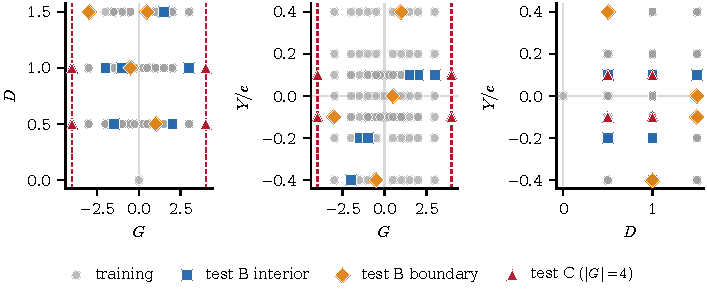
\includegraphics[width=\linewidth]{sections/figures/results/fig_paramspace_v3.pdf}
  \caption{\rb{K}{S2-C3}{Shows the sampling and the symmetric boundary, and names the $Y$ under-sampling that \S5.4 lists as a limitation.}Parameter-space sampling of the $\NCases$ cases in the $(G, D, Y)$ gust
  envelope, shown as three two-dimensional projections and coloured by split:
  training ($\NTrainEnc$ encounters), the stratified in-distribution test set
  ($\NTestBEnc$ encounters from $\NTestBCases$ cases, split into in-distribution
  and edge-of-training tiers), and the $|G| = 4$ extrapolation set
  ($\NTestCEnc$ encounters from $\NTestCCases$ cases). The dashed lines mark the
  $|G| = 4$ extrapolation boundary, now sampled at both signs of the gust so that
  the boundary set is symmetric rather than one-sided. Training mass concentrates
  near $Y/c = 0$, which is why the wall-normal offset is the least well resolved
  parameter (\S\ref{sec:res_latent_physics}).\re}
  \label{fig:paramspace}
\end{figure}
